% ******************************* PhD Thesis Template **************************
% Please have a look at the README.md file for info on how to use the template

\documentclass[a4paper,12pt,times,numbered,print,index]{Classes/PhDThesisPSnPDF}

% ******************************************************************************
% ******************************* Class Options ********************************
% *********************** See README for more details **************************
% ******************************************************************************

% `a4paper'(The University of Cambridge PhD thesis guidelines recommends a page
% size a4 - default option) or `a5paper': A5 Paper size is also allowed as per
% the Cambridge University Engineering Deparment guidelines for PhD thesis
%
% `11pt' or `12pt'(default): Font Size 10pt is NOT recommended by the University
% guidelines
%
% `oneside' or `twoside'(default): Printing double side (twoside) or single
% side.
%
% `print': Use `print' for print version with appropriate margins and page
% layout. Leaving the options field blank will activate Online version.
%
% `index': For index at the end of the thesis
%
% `draft': For draft mode without loading any images (same as draft in book)
%
% `abstract': To generate only the title page and abstract page with
% dissertation title and name, to submit to the Student Registry
%
% `chapter`: This option enables only the specified chapter and it's references
%  Useful for review and corrections.
%
% ************************* Custom Page Margins ********************************
%
% `custommargin`: Use `custommargin' in options to activate custom page margins,
% which can be defined in the preamble.tex. Custom margin will override
% print/online margin setup.
%
% *********************** Choosing the Fonts in Class Options ******************
%
% `times' : Times font with math support. (The Cambridge University guidelines
% recommend using times)
%
% `fourier': Utopia Font with Fourier Math font (Font has to be installed) 
%            It's a free font.
%
% `customfont': Use `customfont' option in the document class and load the
% package in the preamble.tex
%
% default or leave empty: `Latin Modern' font will be loaded.
%
% ********************** Choosing the Bibliography style ***********************
%
% `authoryear': For author-year citation eg., Krishna (2013)
%
% `numbered': (Default Option) For numbered and sorted citation e.g., [1,5,2]
%
% `custombib': Define your own bibliography style in the `preamble.tex' file.
%              `\RequirePackage[square, sort, numbers, authoryear]{natbib}'. 
%              This can be also used to load biblatex instead of natbib 
%              (See Preamble) 
%
% **************************** Choosing the Page Style *************************
%
% `default (leave empty)': For Page Numbers in Header (Left Even, Right Odd) and
% Chapter Name in Header (Right Even) and Section Name (Left Odd). Blank Footer.
%
% `PageStyleI': Chapter Name next & Page Number on Even Side (Left Even).
% Section Name & Page Number in Header on Odd Side (Right Odd). Footer is empty.
%
% `PageStyleII': Chapter Name on Even Side (Left Even) in Header. Section Number
% and Section Name in Header on Odd Side (Right Odd). Page numbering in footer


% ********************************** Preamble **********************************
% Preamble: Contains packages and user-defined commands and settings
% All my custom preamble stuff.  Shouldn't overlap with anything in official-preamble




%\usepackage{bm}  % for warped mixtures - is this necessary?
\usepackage{booktabs}
\usepackage{tabularx}
\usepackage{multirow}
\usepackage{datetime}

% for the list of publications

%\usepackage[resetlabels]{multibib}
\usepackage{bibentry}
%\usepackage{bibunits}
\nobibliography*

\renewcommand{\tabularxcolumn}[1]{>{\arraybackslash}m{#1}}
\usepackage{relsize}
\usepackage{graphicx}
%\usepackage{amsmath,amssymb,textcomp}
\usepackage{nicefrac}
%\usepackage{natbib}
%\usepackage{amsthm}
%\usepackage{algorithm}
%\usepackage{algpseudocode}
\usepackage{tikz}
\usetikzlibrary{bayesnet}
\usepackage{nth}
\usepackage{rotating}
\usepackage{array}
\usepackage{fp}
\usepackage{cleveref}   % Note: this package sometimes causes the page counter to reset.
\crefname{equation}{equation}{equations}
\crefname{figure}{figure}{figures}


\renewcommand{\algorithmicrequire}{\textbf{Input:}}
\renewcommand{\algorithmicensure}{\textbf{Output:}}
%\usepackage{common/sectsty}

% Controls capitalization of all headers
%\usepackage{stringstrings}
%\usepackage[explicit]{titlesec}
%\newcommand\SentenceCase[1]{%
%  \caselower[e]{#1}%
%  \capitalize[q]{\thestring}%
%}
%\titleformat{\section}
%  {\normalfont\Large\bfseries}{\thesection}{1em}{\SentenceCase{#1}\thestring}


%\titleformat{\section} % The normal, unstarred version
%    {\Large\bfseries}{}{2ex}
%    {\thesection. \MakeSentenceCase{#1}}

%\titleformat{name=\section,numberless} % The starred version; note the `numberless` key
%    {\Large\bfseries}{}{2ex}
%    {\MakeSentenceCase{#1}}

\usepackage[hyperpageref]{backref}
% Setup to show (pages 4 and 9) sort of thing in the bibliography - DD
%\def\foo{\hspace{\fill}\mbox{}\linebreak[0]\hspace*{\fill}}
%\def\foo{\parbox{3cm}{\hfill}
%\def\foo{\parbox{3cm}{\hfill}
%\newcommand\foo[1]{{\raggedleft{\hfill{\mbox{\hfill{#1}}}}}}
\newcommand{\comfyfill}[1]{% = Thorsten Donig's \signed
  \unskip\hspace*{0.1em plus 1fill}
  \nolinebreak[3]%
  \hspace*{\fill}\mbox{#1}
  \parfillskip0pt\par
}
\newcommand\foo[1]{{\comfyfill{\mbox{#1}}}}
%\newcommand\foo[1]{{\mbox{#1}}}
\renewcommand*{\backref}[1]{}
\renewcommand*{\backrefalt}[4]{%
\ifcase #1 %
%
\or
\foo{(page #2)}%
\else
\foo{(pages #2)}%
\fi
}

\usepackage{stringstrings}

% Setup TikZ
\usetikzlibrary{arrows,calc,shadings,shapes,shadows,decorations.pathreplacing,positioning}
\tikzstyle{block}=[draw opacity=0.7,line width=1.4cm]
\tikzstyle{every picture}+=[remember picture]
\tikzstyle{na} = [baseline=-.5ex]
\tikzstyle{blockb} = [draw, rectangle, 
minimum height=2em, minimum width=2em]

\pgfdeclarelayer{background}
\pgfdeclarelayer{foreground}
\pgfsetlayers{background,main,foreground}
\tikzstyle{block} = [draw, rectangle, 
minimum height=1em, minimum width=1em]
\tikzstyle{blockg} = [draw, fill=green!20, rectangle, 
minimum height=10em, minimum width=2em, drop shadow]
\tikzstyle{blockr} = [draw, fill=red!20, rectangle, 
minimum height=10em, minimum width=2em, drop shadow]
\tikzstyle{blockb} = [draw, rectangle, 
minimum height=2em, minimum width=2em]
\tikzstyle{sum} = [draw, circle, node distance=1cm]
\tikzstyle{input} = [coordinate]
\tikzstyle{output} = [coordinate]
\tikzstyle{pinstyle} = [pin edge={to-,thin,black}]


%\newcommand{\headercase}{\
%\DeclareFieldFormat{titlecase}{\MakeSentenceCase{#1}}


%% For submission, make all render blank.
%%%%%%%%%%%%%%%%%%%%%%%%%%%%%%%%%%%%%%%%%%%%%%%%%%%%%%%%%%
%%%% EDITING HELPER FUNCTIONS  %%%%%%%%%%%%%%%%%%%%%%%%%%%
%%%%%%%%%%%%%%%%%%%%%%%%%%%%%%%%%%%%%%%%%%%%%%%%%%%%%%%%%%

%% NA: needs attention (rough writing whose correctness needs to be verified)
%% TBD: instructions for how to fix a gap ("Describe the propagation by ...")
%% PROBLEM: bug or missing crucial bit 

%% use \fXXX versions of these macros to put additional explanation into a footnote.  
%% The idea is that we don't want to interrupt the flow of the paper or make it 
%% impossible to read because there are a bunch of comments.

%% NA's (and TBDs, those less crucially) should be written so 
%% that they flow with the text.

\definecolor{WowColor}{rgb}{.75,0,.75}
\definecolor{SubtleColor}{rgb}{0,0,.50}

% inline
\newcommand{\NA}[1]{\textcolor{SubtleColor}{ {\tiny \bf ($\star$)} #1}}
\newcommand{\LATER}[1]{\textcolor{SubtleColor}{ {\tiny \bf ($\dagger$)} #1}}
\newcommand{\TBD}[1]{\textcolor{SubtleColor}{ {\tiny \bf (!)} #1}}
\newcommand{\PROBLEM}[1]{\textcolor{WowColor}{ {\bf (!!)} {\bf #1}}}

% as margin notes

\newcounter{margincounter}
\newcommand{\displaycounter}{{\arabic{margincounter}}}
\newcommand{\incdisplaycounter}{{\stepcounter{margincounter}\arabic{margincounter}}}

\newcommand{\fTBD}[1]{\textcolor{SubtleColor}{$\,^{(\incdisplaycounter)}$}\marginpar{\tiny\textcolor{SubtleColor}{ {\tiny $(\displaycounter)$} #1}}}

\newcommand{\fPROBLEM}[1]{\textcolor{WowColor}{$\,^{((\incdisplaycounter))}$}\marginpar{\tiny\textcolor{WowColor}{ {\bf $\mathbf{((\displaycounter))}$} {\bf #1}}}}

\newcommand{\fLATER}[1]{\textcolor{SubtleColor}{$\,^{(\incdisplaycounter\dagger)}$}\marginpar{\tiny\textcolor{SubtleColor}{ {\tiny $(\displaycounter\dagger)$} #1}}}

%\renewcommand{\LATER}[1]{}
%\renewcommand{\fLATER}[1]{}
%\renewcommand{\TBD}[1]{}
%\renewcommand{\fTBD}[1]{}
%\renewcommand{\PROBLEM}[1]{}
%\renewcommand{\fPROBLEM}[1]{}
%\renewcommand{\NA}[1]{}


% HUMBLE WORDS: shown slightly smaller when in normal text
% Thanks to Christian Steinruecken!

% HUMBLE WORDS: shown slightly smaller when in normal text
% Christian Steinruecken
%
\makeatletter%
%\def\@humbleformat#1{{\fontsize{}{1em}\selectfont #1}}
%\def\@humbleformat#1{\textsmaller{#1}}%
\newlength{\nonHumbleHeight}
\def\@humbleformat#1{{\settoheight{\nonHumbleHeight}{#1}\resizebox{!}{0.94\nonHumbleHeight}{#1}}}%
\def\@idxhumbleformat#1{{\relscale{0.95}{#1}}}%
%\def\@humbleformat#1{{#1}}%
\def\declareHumble#1#2{%
  \expandafter\def\csname #1\endcsname{\@humbleformat{#2}}%
  \expandafter\def\csname s#1\endcsname{{#2}}%
  \expandafter\def\csname idx#1\endcsname{{\@idxhumbleformat{#2}}}%
}%
\def\humble#1{\@humbleformat{#1}}%
\def\idxhumble#1{\@idxhumbleformat{#1}}%
\makeatother%

% Convenient indexing for humble abbreviations
\def\humbleindex#1#2{\index{#1@\idxhumble{#1}}}


\def\subexpr{{\cal S}}
\def\baseker{{\cal B}}
\def\numWinners{k}

\def\ie{i.e.\ }
\def\eg{e.g.\ }
\def\etc{etc.\ }
\let\oldemptyset\emptyset
%\let\emptyset 0

\DeclareMathOperator{\erf}{erf} 
\DeclareMathOperator{\real}{Re}
\DeclareMathOperator{\imag}{Im} 
\DeclareMathOperator{\tr}{tr}
\DeclareMathOperator{\cov}{cov} 
\DeclareMathOperator{\ex}{\mathbb{E}}
\DeclareMathOperator{\var}{var}
\DeclareMathOperator{\bdiag}{blockdiag}
\DeclareMathOperator{\vecO}{vec} \DeclareMathOperator{\diag}{diag}
\DeclareMathOperator{\const}{const}
\DeclareMathOperator{\entropy}{H}
\providecommand{\abs}[1]{\lvert#1\rvert}

\renewcommand{\Re}{\mathbb{R}}

\newcommand{\boldt}{\mathbf{t}}
\newcommand{\boldw}{\mathbf{w}}
\newcommand{\bolde}{\mathbf{e}}
\newcommand{\bolds}{\mathbf{s}}
\newcommand{\boldy}{\mathbf{y}} % output space
\newcommand{\boldx}{\mathbf{x}} % input space of the outputs
\newcommand{\boldz}{\mathbf{z}} % input space of the latent functions
\newcommand{\boldh}{\mathbf{h}} % lag
\newcommand{\boldk}{\mathbf{k}} % kernel or covariance
\newcommand{\boldf}{\mathbf{f}} % outputs without noise
\newcommand{\boldu}{\mathbf{u}} % vector for latent function
\newcommand{\bolda}{\mathbf{a}} % vector for SLFM function
\newcommand{\boldl}{\mathbf{l}} % vector for lenghtscales
\newcommand{\boldm}{\mathbf{m}} % vector for means
\newcommand{\boldg}{\mathbf{g}} % vector for means
\newcommand{\boldb}{\mathbf{b}} % vector for means
\newcommand{\boldJ}{\mathbf{J}} % vector for means

\newcommand{\boldbeta}{\bm{\beta}}
\newcommand{\boldpsi}{\bm{\psi}}
\newcommand{\boldPsi}{\bm{\Psi}}
\newcommand{\boldmu}{\bm{\mu}}
\newcommand{\boldgamma}{\bm{\gamma}}
\newcommand{\boldsigma}{\bm{\sigma}}
\newcommand{\boldlambda}{\bm{\lambda}}
\newcommand{\boldSigma}{\bm{\Sigma}}
\newcommand{\boldUpsi}{\bm{\Upsilon}}% vector of coefficients in th IMC
\newcommand{\boldupsi}{\bm{\upsilon}}% vector of coefficients in th IMC
\newcommand{\boldtheta}{\bm{\theta}}% vector of coefficients in th IMC
\newcommand{\boldepsilon}{\bm{\epsilon}}
\newcommand{\boldGamma}{\bm{\Gamma}}

\newcommand{\LowerBound}{\mathcal{F}}

%Operators
\DeclareMathOperator{\deriv}{d} 
\DeclareMathOperator{\dif}{d}
\DeclareMathOperator*{\argmin}{arg\,min}
\DeclareMathOperator*{\argmax}{arg\,max}

%State space Matrices
\newcommand{\boldA}{\mathbf{A}} % matrix of dynamics
\newcommand{\boldB}{\mathbf{B}} % matrix of excitation 
\newcommand{\boldC}{\mathbf{C}}

\newcommand{\boldQ}{\mathbf{Q}}
\newcommand{\boldF}{\mathbf{F}}
\newcommand{\boldL}{\mathbf{L}}
\newcommand{\boldH}{\mathbf{H}} %
\newcommand{\boldq}{\mathbf{q}} % 
\newcommand{\boldr}{\mathbf{r}} % 
\newcommand{\boldR}{\mathbf{R}} % 
\newcommand{\boldv}{\mathbf{v}} % 

\newcommand{\boldG}{\mathbf{G}}
\newcommand{\boldK}{\mathbf{K}} % kernel or covariance
\newcommand{\boldZ}{\mathbf{Z}}
\newcommand{\boldS}{\mathbf{S}}
\newcommand{\boldX}{\mathbf{X}} % The whole set of input vectors
\newcommand{\boldI}{\mathbf{I}} % The identity matrix
\newcommand{\boldP}{\mathbf{P}} % coregionalization matrix
\newcommand{\boldM}{\mathbf{M}} % coregionalization matrix


\newcommand{\boldAtilde}{\mathbf{\widetilde{A}}} % vector for SL\boldK_{\boldu,\boldu}^{-1}\widetilde{\boldK}_{\boldu,\boldu}\boldK_{\boldu,\boldu}^{-1}FM function
\newcommand{\inputSpace}{\mathcal{X}} % The input space
\newcommand{\eye}{\mathbf{I}}   % identity matrix

\newcommand{\params}{\bm{\theta}} % Parameters of LMC model
\newcommand{\veC}{\textbf{\hspace{-0.001in}:}} % Simplified version of the vec operator (vec = :)
\newcommand{\preci}{\mathbf{P}}% Precision for the Gaussians
\newcommand{\dataset}{{\cal D}} % dataset
\newcommand{\gauss}{\mathcal{N}} % Gaussian density
\newcommand{\gammad}{\operatorname{Gamma}} % Gamma density
\newcommand{\betad}{\operatorname{Beta}} % Beta density
\newcommand{\bernd}{\operatorname{Bernoulli}} % Bernoulli density
\newcommand{\ones}{\mathbf{1}}
\newcommand{\zeros}{\mathbf{0}}

\newcommand\Tau{\mathcal{T}}% Caligraphic T for example
\newcommand{\fracpartial}[2]{\frac{\partial #1}{\partial #2}}


%%%%% my maths definitions

%\newcommand{\tr}{\operatorname{tr}}
\newcommand{\gD}[2]{\mathcal{N}\left(#1,#2\right)}
\newcommand{\dWj}{\partial\projMat}
\newcommand{\kernel}[2]{k\left(#1,#2\right)}
\newcommand{\kernelww}[2]{k\left(\mathbf{w}_{#1}^v,\mathbf{w}_{#2}^d\right)}
\newcommand{\kernelwx}[1]{k\left(\mathbf{w}_{#1}^v,\indobj\right)}
\newcommand{\catD}[2]{\mathcal{G}\left(#1,#2\right)}
\newcommand{\Z}{\boldsymbol{\mathrm{Z}}}
%\newcommand{\C}{\boldsymbol{\Lambda}_j}
\newcommand{\Cin}{\mathbf{C}_j}
\newcommand{\Cnl}{\boldsymbol{\Lambda}_j}
\newcommand{\muJ}{\boldsymbol{\mu}_j}
\newcommand{\gammaA}{\Gamma\left(a\right)}
%\newcommand{\eye}{\mathbf{I}}
\newcommand{\Scluster}{\mathbf{S}}
\newcommand{\W}{\boldsymbol{\mathcal{W}}}

\newcommand{\WIn}{\mathbf{W}}

\newcommand{\setX}{\mathbf{X}}
\newcommand{\setXphi}{\boldsymbol{\Phi}}
\newcommand{\setObj}{\mathbf{X}_v}
%\newcommand{\setObj}{\mathbf{X}_d}
\newcommand{\setObjH}{\bm{\Phi}_v}
%\newcommand{\indobj}{\mathbf{x}_{dn}}
\newcommand{\indobj}{\mathbf{x}_{vn}}
\newcommand{\indobjm}{\mathbf{x}_{vm}}

%\newcommand{\projMat}{\boldsymbol{\mathcal{W}}_d}
\newcommand{\projMat}{\bm{B}_v}

\newcommand{\projMatI}{\mathbf{W}_v}
\newcommand{\dWjIn}{\partial\projMatI}
\newcommand{\lvecI}{\mathbf{z}_j}
\newcommand{\lvecsI}{\mathbf{z}_{s_{vn}}}
\newcommand{\lvec}{\boldsymbol{\zeta}_j}
\newcommand{\lvecs}{\boldsymbol{\zeta}_{s_{vn}}}
\newcommand{\mixwe}{{\theta}_j}
\newcommand{\mapphi}{\phi\left(x\right)}
\newcommand{\mapphit}{\phi\left(x'\right)}
\newcommand{\comment}[2]{{\color{blue}#1} {\color{red}#2}}
\newcommand{\phixnd}{\boldsymbol{\phi}\left(\indobj\right)}
\newcommand{\phixmd}{\boldsymbol{\phi}\left(\indobjm\right)}
\newcommand{\phiwld}[1]{\boldsymbol{\varphi}\left(\mathbf{w}_{#1}^d\right)}
\newcommand{\phiwldI}[2]{\varphi_{#2}\left(\mathbf{w}_{#1}^v\right)}
\newcommand{\wH}{\boldsymbol{\omega}_{j}^v}
\newcommand{\wHj}[1]{\boldsymbol{\omega}_{#1}^v}
\newcommand{\wIj}[1]{\mathbf{w}_{#1}^v}
\newcommand{\muJFa}{\sum_{v=1}^{V}\mathbf{\hat{k}}_v }
\newcommand{\kawx}{\mathbf{\hat{k}}_v }
\newcommand{\Kaww}{\mathbf{\hat{K}}_v }
\newcommand{\Kv}{\mathbf{K}_v }
\newcommand{\dWd}{\partial \boldsymbol{\Theta}}
\newcommand{\phix}{\bm{\phi}\left(\mathbf{x}\right)}
\newcommand{\phixp}{\bm{\phi}\left(\mathbf{x}^\prime\right)}

%% multiview model
\newcommand{\setWv}{\mathbf{W}^{v}}
\newcommand{\setYv}{\mathbf{Y}_{v}}
\newcommand{\setY}{\mathbf{Y}}
\newcommand{\setZ}{\mathbf{Z}}
\newcommand{\setSv}{\mathbf{S}_{v}}
\newcommand{\setXv}{\mathbf{X}_{v}}
\newcommand{\setZv}{\mathbf{Z}_{v}}
\newcommand{\setFv}{\mathbf{F}_{v}}
\newcommand{\setKv}{\mathbf{K}_{v}}
\newcommand{\hParams}{\boldsymbol{\theta}}
\newcommand{\hParamsv}{\boldsymbol{\theta}^{v}}
\newcommand{\obspv}{\mathbf{x}_{nv}}
\newcommand{\lambdac}{\lambda_c}
\newcommand{\muC}{\boldsymbol{\mu}_c}
\newcommand{\RC}{\mathbf{R}_c}
\newcommand{\Cnlc}{\boldsymbol{\Lambda}_c}
\newcommand{\Cnlw}{\boldsymbol{\Lambda}}

\newcommand{\likel}{\log p\left(\boldsymbol{\Phi},\mathbf{S}|\W,a,b,r,\gamma\right)}
\newcommand{\GP}[2]{\mathcal{GP}\left(#1,#2\right)}

%\counterwithout*{footnote}{chapter}


% ************************ Thesis Information & Meta-data **********************
% Thesis title and author information, refernce file for biblatex
% ************************ Thesis Information & Meta-data **********************

%% The title of the thesis
\title{Thesis Title}



%\texorpdfstring is used for PDF metadata. Usage:
%\texorpdfstring{LaTeX_Version}{PDF Version (non-latex)} eg.,
%\texorpdfstring{$sigma$}{sigma}

%% The full name of the author
\author{Author's Full Name}

%% Department (eg. Department of Engineering, Maths, Physics)
%\dept{Department of Engineering}

%% University and Crest
\university{Universidad de Antioquia}
\crest{
\includegraphics[width=0.3\textwidth]{misc/lodoUdeA1}}

%% You can redefine the submission text:
% Default as per the University guidelines: This dissertation is submitted for
% the degree of Doctor of Philosophy
%\renewcommand{\submissiontext}{change the default text here if needed}

%% Full title of the Degree 
\degree{Doctor of Engineering}
 
%% College affiliation (optional)
\college{Research Group}

%% Submission date
\degreedate{} 

%% Meta information
\subject{Thesis's Topic}
\keywords{{LaTeX} {PhD Thesis} {Engineering} {Universidad de Antioquia}}



% ***************************** Abstract Separate ****************************** 
% To printout only the titlepage and the abstract with the PhD title and the 
% author name for submission to the Student Registry, use the `abstract' option in
% the document class. 

\ifdefineAbstract
 \pagestyle{empty}
 \includeonly{Declaration/declaration, Abstract/abstract} 
\fi

% ***************************** Chapter Mode ***********************************
% The chapter mode allows user to only print particular chapters with references
% Title, Contents, Frontmatter are disabled by default
% Useful option to review a particular chapter or to send it to supervisior.
% To use choose `chapter' option in the document class

\ifdefineChapter
 \includeonly{Chapter3/chapter3} 
\fi

% ******************************** Front Matter ********************************
\begin{document}

\frontmatter

\begin{titlepage}

\maketitle

\end{titlepage}

% ******************************* Thesis Dedidcation ********************************

\begin{dedication} 

I would like to dedicate this thesis to my loving parents ...

\end{dedication}


% ******************************* Thesis Declaration ********************************

\begin{declaration}

I hereby declare that except where specific reference is made to the work of others, the contents of this dissertation are original and have not been submitted in whole or in part for consideration for any other degree or qualification in this, or any other University. This dissertation is the result of my own work and includes nothing which is the outcome of work done in collaboration, except where specifically indicated in the text. This dissertation contains less than 65,000 words including appendices, bibliography, footnotes, tables and equations and has less than 150 figures.

% Author and date will be inserted automatically from thesis.tex \author \degreedate

\end{declaration}


% ************************** Thesis Acknowledgements *****************************

\begin{acknowledgements}      


And I would like to acknowledge ...


\end{acknowledgements}

% ************************** Thesis Abstract *****************************
% Use `abstract' as an option in the document class to print only the titlepage and the abstract.
\begin{abstract}
This is where you write your abstract ...
\end{abstract}


% *********************** Adding TOC and List of Figures ***********************

\tableofcontents

\listoffigures

\listoftables 

% \printnomenclature[space] space can be set as 2.5cm between symbol and
% description
\printnomencl

% ******************************** Main Matter *********************************
\mainmatter

%*****************************************************************************************
%*********************************** First Chapter ***************************************
%*****************************************************************************************

\chapter{Getting Started}  %Title of the First Chapter

\ifpdf
    \graphicspath{{Chapter1/Figs/Raster/}{Chapter1/Figs/PDF/}{Chapter1/Figs/}}
\else
    \graphicspath{{Chapter1/Figs/Vector/}{Chapter1/Figs/}}
\fi


%********************************** %First Section  **************************************
\section{What is Loren Ipsum? Title with Math \texorpdfstring{$\sigma$}{[sigma]}} %Section - 1.1 

Lorem Ipsum is simply dummy text of the printing and typesetting industry (see Section~\ref{section1.3}). Lorem Ipsum~\citep{Aup91} has been the industry's standard dummy text ever since the 1500s, when an unknown printer took a galley of type and scrambled it to make a type specimen book. It has survived not only five centuries, but also the leap into electronic typesetting, remaining essentially unchanged. It was popularised in the 1960s with the release of Letraset sheets containing Lorem Ipsum passages, and more recently with desktop publishing software like Aldus PageMaker including versions of Lorem Ipsum~\citep{AAB95,Con90,LM65}.

The most famous equation in the world: $E^2 = (m_0c^2)^2 + (pc)^2$, which is known as the \textbf{energy-mass-momentum} relation as an in-line equation.

A {\em \LaTeX{} class file}\index{\LaTeX{} class file@LaTeX class file} is a file, which holds style information for a particular \LaTeX{}.

\begin{eqnarray}
CIF: \hspace*{5mm}F_0^j(a) &=& \frac{1}{2\pi \iota} \oint_{\gamma} \frac{F_0^j(z)}{z - a} dz
\end{eqnarray}

\nomenclature[z-cif]{$CIF$}{Cauchy's Integral Formula}                                % first letter Z is for Acronyms 
\nomenclature[a-F]{$F$}{complex function}                                                   % first letter A is for Roman symbols
\nomenclature[g-p]{$\pi$}{ $\simeq 3.14\ldots$}                                             % first letter G is for Greek Symbols
\nomenclature[g-i]{$\iota$}{unit imaginary number $\sqrt{-1}$}                      % first letter G is for Greek Symbols
\nomenclature[g-g]{$\gamma$}{a simply closed curve on a complex plane}  % first letter G is for Greek Symbols
\nomenclature[x-i]{$\oint_\gamma$}{integration around a curve $\gamma$} % first letter X is for Other Symbols
\nomenclature[r-j]{$j$}{superscript index}                                                       % first letter R is for superscripts
\nomenclature[s-0]{$0$}{subscript index}                                                        % first letter S is for subscripts


%********************************** %Second Section  *************************************
\section{Why do we use Loren Ipsum?} %Section - 1.2


It is a long established fact that a reader will be distracted by the readable content of a page when looking at its layout. The point of using Lorem Ipsum is that it has a more-or-less normal distribution of letters, as opposed to using `Content here, content here', making it look like readable English. Many desktop publishing packages and web page editors now use Lorem Ipsum as their default model text, and a search for `lorem ipsum' will uncover many web sites still in their infancy. Various versions have evolved over the years, sometimes by accident, sometimes on purpose (injected humour and the like).

%********************************** % Third Section  *************************************
\section{Where does it come from?}  %Section - 1.3 
\label{section1.3}

Contrary to popular belief, Lorem Ipsum is not simply random text. It has roots in a piece of classical Latin literature from 45 BC, making it over 2000 years old. Richard McClintock, a Latin professor at Hampden-Sydney College in Virginia, looked up one of the more obscure Latin words, consectetur, from a Lorem Ipsum passage, and going through the cites of the word in classical literature, discovered the undoubtable source. Lorem Ipsum comes from sections 1.10.32 and 1.10.33 of "de Finibus Bonorum et Malorum" (The Extremes of Good and Evil) by Cicero, written in 45 BC. This book is a treatise on the theory of ethics, very popular during the Renaissance. The first line of Lorem Ipsum, "Lorem ipsum dolor sit amet..", comes from a line in section 1.10.32.

The standard chunk of Lorem Ipsum used since the 1500s is reproduced below for those interested. Sections 1.10.32 and 1.10.33 from ``de Finibus Bonorum et Malorum" by Cicero are also reproduced in their exact original form, accompanied by English versions from the 1914 translation by H. Rackham

``Lorem ipsum dolor sit amet, consectetur adipisicing elit, sed do eiusmod tempor incididunt ut labore et dolore magna aliqua. Ut enim ad minim veniam, quis nostrud exercitation ullamco laboris nisi ut aliquip ex ea commodo consequat. Duis aute irure dolor in reprehenderit in voluptate velit esse cillum dolore eu fugiat nulla pariatur. Excepteur sint occaecat cupidatat non proident, sunt in culpa qui officia deserunt mollit anim id est laborum."

Section 1.10.32 of ``de Finibus Bonorum et Malorum", written by Cicero in 45 BC: ``Sed ut perspiciatis unde omnis iste natus error sit voluptatem accusantium doloremque laudantium, totam rem aperiam, eaque ipsa quae ab illo inventore veritatis et quasi architecto beatae vitae dicta sunt explicabo. Nemo enim ipsam voluptatem quia voluptas sit aspernatur aut odit aut fugit, sed quia consequuntur magni dolores eos qui ratione voluptatem sequi nesciunt. Neque porro quisquam est, qui dolorem ipsum quia dolor sit amet, consectetur, adipisci velit, sed quia non numquam eius modi tempora incidunt ut labore et dolore magnam aliquam quaerat voluptatem. Ut enim ad minima veniam, quis nostrum exercitationem ullam corporis suscipit laboriosam, nisi ut aliquid ex ea commodi consequatur? Quis autem vel eum iure reprehenderit qui in ea voluptate velit esse quam nihil molestiae consequatur, vel illum qui dolorem eum fugiat quo voluptas nulla pariatur?"

1914 translation by H. Rackham: ``But I must explain to you how all this mistaken idea of denouncing pleasure and praising pain was born and I will give you a complete account of the system, and expound the actual teachings of the great explorer of the truth, the master-builder of human happiness. No one rejects, dislikes, or avoids pleasure itself, because it is pleasure, but because those who do not know how to pursue pleasure rationally encounter consequences that are extremely painful. Nor again is there anyone who loves or pursues or desires to obtain pain of itself, because it is pain, but because occasionally circumstances occur in which toil and pain can procure him some great pleasure. To take a trivial example, which of us ever undertakes laborious physical exercise, except to obtain some advantage from it? But who has any right to find fault with a man who chooses to enjoy a pleasure that has no annoying consequences, or one who avoids a pain that produces no resultant pleasure?"

Section 1.10.33 of ``de Finibus Bonorum et Malorum", written by Cicero in 45 BC: ``At vero eos et accusamus et iusto odio dignissimos ducimus qui blanditiis praesentium voluptatum deleniti atque corrupti quos dolores et quas molestias excepturi sint occaecati cupiditate non provident, similique sunt in culpa qui officia deserunt mollitia animi, id est laborum et dolorum fuga. Et harum quidem rerum facilis est et expedita distinctio. Nam libero tempore, cum soluta nobis est eligendi optio cumque nihil impedit quo minus id quod maxime placeat facere possimus, omnis voluptas assumenda est, omnis dolor repellendus. Temporibus autem quibusdam et aut officiis debitis aut rerum necessitatibus saepe eveniet ut et voluptates repudiandae sint et molestiae non recusandae. Itaque earum rerum hic tenetur a sapiente delectus, ut aut reiciendis voluptatibus maiores alias consequatur aut perferendis doloribus asperiores repellat."

1914 translation by H. Rackham: ``On the other hand, we denounce with righteous indignation and dislike men who are so beguiled and demoralized by the charms of pleasure of the moment, so blinded by desire, that they cannot foresee the pain and trouble that are bound to ensue; and equal blame belongs to those who fail in their duty through weakness of will, which is the same as saying through shrinking from toil and pain. These cases are perfectly simple and easy to distinguish. In a free hour, when our power of choice is untrammelled and when nothing prevents our being able to do what we like best, every pleasure is to be welcomed and every pain avoided. But in certain circumstances and owing to the claims of duty or the obligations of business it will frequently occur that pleasures have to be repudiated and annoyances accepted. The wise man therefore always holds in these matters to this principle of selection: he rejects pleasures to secure other greater pleasures, or else he endures pains to avoid worse pains."

%*****************************************************************************************
%*********************************** Second Chapter **************************************
%*****************************************************************************************

\chapter{My Second Chapter}

\ifpdf
    \graphicspath{{Chapter2/Figs/Raster/}{Chapter2/Figs/PDF/}{Chapter2/Figs/}}
\else
    \graphicspath{{Chapter2/Figs/Vector/}{Chapter2/Figs/}}
\fi


\section[Short title]{Reasonably Long Section Title}

% Uncomment this line, when you have siunitx package loaded.
%The SI Units for dynamic viscosity is \si{\newton\second\per\metre\squared}.
I'm going to randomly include a picture Figure~\ref{fig:minion}.


If you have trouble viewing this document contact Krishna \href{mailto:kks32@cam.ac.uk}{kks32@cam.ac.uk}. 


\begin{figure}[htbp!] 
\centering    

\includegraphics[width=1.0\textwidth]{minion}
\caption[Minion]{This is just a long figure caption for the minion in Despicable Me from Pixar}
\label{fig:minion}
\end{figure}


\section*{Enumeration}
\begin{enumerate}
\item The first topic is dull
\item The second topic is duller
\begin{enumerate}
\item The first subtopic is silly
\item The second subtopic is stupid
\end{enumerate}
\item The third topic is dullest
\end{enumerate}

\section*{itemize}
\begin{itemize}
\item The first topic is dull
\item The second topic is duller
\begin{itemize}
\item The first subtopic is silly
\item The second subtopic is stupid
\end{itemize}
\item The third topic is dullest
\end{itemize}

\section*{description}
\begin{description}
\item[The first topic] is dull
\item[The second topic] is duller
\begin{description}
\item[The first subtopic] is silly
\item[The second subtopic] is stupid
\end{description}
\item[The third topic] is dullest
\end{description}


\clearpage

\tochide\section{Hidden Section}
\textbf{Lorem ipsum dolor sit amet}, \textit{consectetur adipiscing elit}. In magna nisi, aliquam id blandit id, congue ac est. Fusce porta consequat leo. Proin feugiat at felis vel consectetur. Ut tempus ipsum sit amet congue posuere. Nulla varius rutrum quam. Donec sed purus luctus, faucibus velit id, ultrices sapien. Cras diam purus, tincidunt eget tristique ut, egestas quis nulla. Curabitur vel iaculis lectus. Nunc nulla urna, ultrices et eleifend in, accumsan ut erat. In ut ante leo. Aenean a lacinia nisl, sit amet ullamcorper dolor. Maecenas blandit, tortor ut scelerisque congue, velit diam volutpat metus, sed vestibulum eros justo ut nulla. Etiam nec ipsum non enim luctus porta in in massa. Cras arcu urna, malesuada ut tellus ut, pellentesque mollis risus.Morbi vel tortor imperdiet arcu auctor mattis sit amet eu nisi. Nulla gravida urna vel nisl egestas varius. Aliquam posuere ante quis malesuada dignissim. Mauris ultrices tristique eros, a dignissim nisl iaculis nec. Praesent dapibus tincidunt mauris nec tempor. Curabitur et consequat nisi. Quisque viverra egestas risus, ut sodales enim blandit at. Mauris quis odio nulla. Cras euismod turpis magna, in facilisis diam congue non. Mauris faucibus nisl a orci dictum, et tempus mi cursus.

Etiam elementum tristique lacus, sit amet eleifend nibh eleifend sed \footnote{My footnote goes blah blah blah! \dots}. Maecenas dapibu augue ut urna malesuada, non tempor nibh mollis. Donec sed sem sollicitudin, convallis velit aliquam, tincidunt diam. In eu venenatis lorem. Aliquam non augue porttitor tellus faucibus porta et nec ante. Proin sodales, libero vitae commodo sodales, dolor nisi cursus magna, non tincidunt ipsum nibh eget purus. Nam rutrum tincidunt arcu, tincidunt vulputate mi sagittis id. Proin et nisi nec orci tincidunt auctor et porta elit. Praesent eu dolor ac magna cursus euismod. Integer non dictum nunc.


\begin{landscape}

\section*{Subplots}
I can cite Wall-E (see Fig.~\ref{fig:WallE}) and Minions in despicable me (Fig.~\ref{fig:Minnion}) or I can cite the whole figure as Fig.~\ref{fig:animations}


\begin{figure}
  \centering
  \subfloat[A Tom and Jerry]{\label{fig:TomJerry}
\includegraphics[width=0.3\textwidth]{TomandJerry}}                
  \subfloat[A Wall-E]{\label{fig:WallE}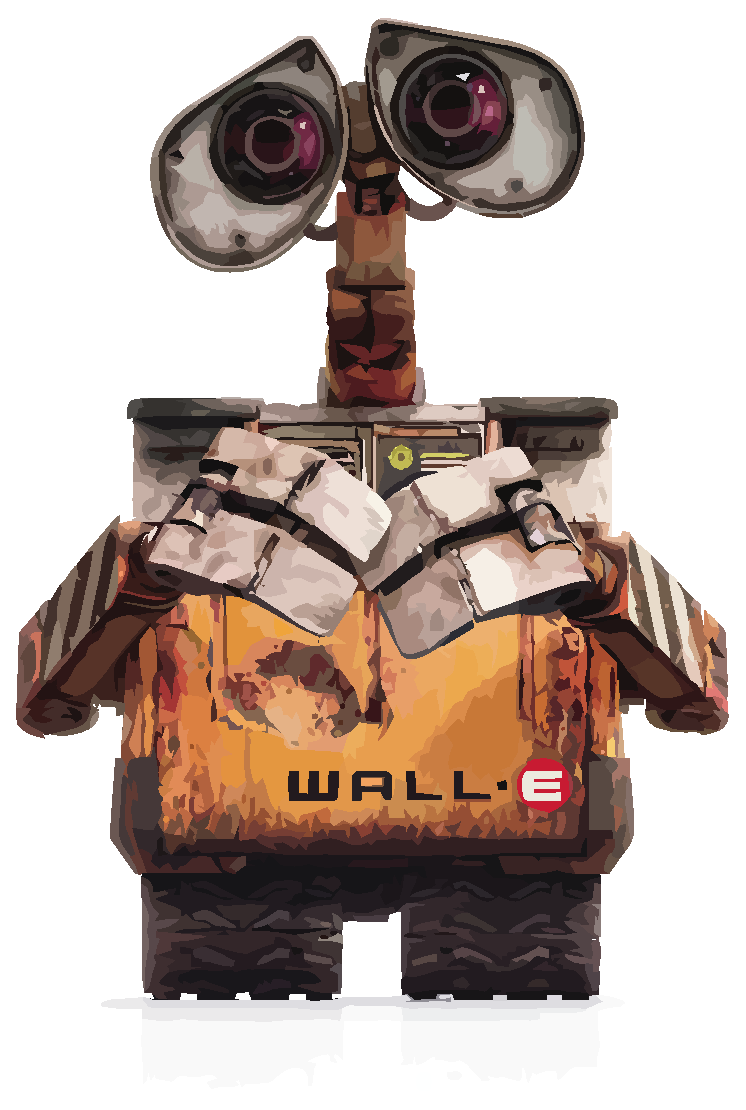
\includegraphics[width=0.3\textwidth]{WallE}}
  \subfloat[A Minion]{\label{fig:Minnion}
\includegraphics[width=0.3\textwidth]{minion}}
  \caption{Best Animations}
  \label{fig:animations}
\end{figure}


\end{landscape}

\chapter{My Third Chapter}

% **************************** Define Graphics Path **************************
\ifpdf
    \graphicspath{{Chapter3/Figs/Raster/}{Chapter3/Figs/PDF/}{Chapter3/Figs/}}
\else
    \graphicspath{{Chapter3/Figs/Vector/}{Chapter3/Figs/}}
\fi

\section{First Section of the Third Chapter}
And now I begin my third chapter here \dots

And now to cite some more people~\citet{Rea85,Ancey1996}

\subsection{First Subsection in the First Section}
\dots and some more 

\subsection{Second Subsection in the First Section}
\dots and some more \dots

\subsubsection{First subsub section in the second subsection}
\dots and some more in the first subsub section otherwise it all looks the same
doesn't it? well we can add some text to it \dots

\subsection{Third Subsection in the First Section}
\dots and some more \dots

\subsubsection{First subsub section in the third subsection}
\dots and some more in the first subsub section otherwise it all looks the same
doesn't it? well we can add some text to it and some more and some more and
some more and some more and some more and some more and some more \dots

\subsubsection{Second subsub section in the third subsection}
\dots and some more in the first subsub section otherwise it all looks the same
doesn't it? well we can add some text to it \dots

\section{Second Section of the Third Chapter}
and here I write more \dots

Now we can refer to the table using Table.~\ref{t:borders}.
\begin{table}[h]
\caption{Table with Borders}
\centering
\label{t:borders}
\begin{tabular}{|l|c| r|}

\hline
1 & 2 & 3 \\ \hline
4 & 5 & 6 \\ \hline
7 & 8 & 9 \\ \hline
\end{tabular}
\end{table}

%\input{Chapter4/chapter4}
%\input{Chapter5/chapter5}
%\input{Chapter6/chapter6}
%\input{Chapter7/chapter7}



% ********************************** Back Matter *******************************
% Backmatter should be commented out, if you are using appendices after References
%\backmatter 

% ********************************** Bibliography ******************************
\begin{spacing}{0.9}

% To use the conventional natbib style referencing
% Bibliography style previews: http://nodonn.tipido.net/bibstyle.php

\bibliographystyle{apalike}
%%\bibliographystyle{plainnat} % use this to have URLs listed in References
\cleardoublepage
\bibliography{References/references} % Path to your References.bib file


% If you would like to use BibLaTeX for your references, pass `custombib' as 
% an option in the document class. The location of 'reference.bib' should be 
% specified in the preamble.tex file in the custombib section. 
% Comment out the lines related to natbib above and uncomment the following line.

% \printbibliography[heading=bibintoc, title={References}]


\end{spacing}

% ********************************** Appendices ********************************

\begin{appendices} % Using appendices environment for more functunality

% ******************************* Thesis Appendix A ********************************
\chapter{How to install \LaTeX} 

\section*{Windows OS}

\subsection*{TeXLive package - full version}
\begin{enumerate}
\item	Download the TeXLive ISO (2.2GB) from\\
\href{https://www.tug.org/texlive/}{https://www.tug.org/texlive/}
\item	Download WinCDEmu (if you don't have a virtual drive) from \\
\href{http://wincdemu.sysprogs.org/download/}{http://wincdemu.sysprogs.org/download/}
\item	To install Windows CD Emulator follow the instructions at\\
\href{http://wincdemu.sysprogs.org/tutorials/install/}{http://wincdemu.sysprogs.org/tutorials/install/}
\item	Right click the iso and mount it using the WinCDEmu as shown in \\
\href{http://wincdemu.sysprogs.org/tutorials/mount/}{http://wincdemu.sysprogs.org/tutorials/mount/}
\item	Open your virtual drive and run setup.pl
\end{enumerate}

or

\subsection*{Basic MikTeX - TeX distribution}
\begin{enumerate}
\item	Download Basic-MiK\TeX (32bit or 64bit) from\\
\href{http://miktex.org/download}{http://miktex.org/download}
\item	Run the installer 
\item	To add a new package go to Start >> All Programs >> MikTex >> Maintenance (Admin) and choose Package Manager
\item	Select or search for packages to install
\end{enumerate}

\subsection*{TexStudio - Tex Editor}
\begin{enumerate}
\item	Download TexStudio from\\
\href{http://texstudio.sourceforge.net/\#downloads}{http://texstudio.sourceforge.net/\#downloads} 
\item	Run the installer
\end{enumerate}

\section*{Mac OS X}
\subsection*{MacTeX - TeX distribution}
\begin{enumerate}
\item	Download the file from\\
\href{https://www.tug.org/mactex/}{https://www.tug.org/mactex/}
\item	Extract and double click to run the installer. It does the entire configuration, sit back and relax.
\end{enumerate}

\subsection*{TexStudio - Tex Editor}
\begin{enumerate}
\item	Download TexStudio from\\
\href{http://texstudio.sourceforge.net/\#downloads}{http://texstudio.sourceforge.net/\#downloads} 
\item	Extract and Start
\end{enumerate}


\section*{Unix/Linux}
\subsection*{TeXLive - TeX distribution}
\subsubsection*{Getting the distribution:}
\begin{enumerate}
\item	TexLive can be downloaded from\\
\href{http://www.tug.org/texlive/acquire-netinstall.html}{http://www.tug.org/texlive/acquire-netinstall.html}.
\item	TexLive is provided by most operating system you can use (rpm,apt-get or yum) to get TexLive distributions
\end{enumerate}

\subsubsection*{Installation}
\begin{enumerate}
\item	Mount the ISO file in the mnt directory
\begin{verbatim}
mount -t iso9660 -o ro,loop,noauto /your/texlive####.iso /mnt
\end{verbatim}

\item	Install wget on your OS (use rpm, apt-get or yum install)
\item	Run the installer script install-tl.
\begin{verbatim}
	cd /your/download/directory
	./install-tl
\end{verbatim}
\item	Enter command `i' for installation

\item	Post-Installation configuration:\\
\href{http://www.tug.org/texlive/doc/texlive-en/texlive-en.html\#x1-320003.4.1}{http://www.tug.org/texlive/doc/texlive-en/texlive-en.html\#x1-320003.4.1} 
\item	Set the path for the directory of TexLive binaries in your .bashrc file
\end{enumerate}

\subsubsection*{For 32Bit OS}
For Bourne-compatible shells such as bash, and using Intel x86 GNU/Linux and a default directory setup as an example, the file to edit might be \begin{verbatim}
edit $~/.bashrc file and add following lines
PATH=/usr/local/texlive/2011/bin/i386-linux:$PATH; 
export PATH 
MANPATH=/usr/local/texlive/2011/texmf/doc/man:$MANPATH;
export MANPATH 
INFOPATH=/usr/local/texlive/2011/texmf/doc/info:$INFOPATH;
export INFOPATH
\end{verbatim}
\subsubsection*{For 64Bit}
\begin{verbatim}
edit $~/.bashrc file and add following lines
PATH=/usr/local/texlive/2011/bin/x86_64-linux:$PATH;
export PATH 
MANPATH=/usr/local/texlive/2011/texmf/doc/man:$MANPATH;
export MANPATH 
INFOPATH=/usr/local/texlive/2011/texmf/doc/info:$INFOPATH;
export INFOPATH

\end{verbatim}



%\subsection{Installing directly using Linux packages} 
\subsubsection*{Fedora/RedHat/CENTOS:}
\begin{verbatim} 
sudo yum install texlive 
sudo yum install psutils 
\end{verbatim}


\subsubsection*{SUSE:}
\begin{verbatim}
sudo zypper install texlive
\end{verbatim}


\subsubsection*{Debian/Ubuntu:}
\begin{verbatim} 
sudo apt-get install texlive texlive-latex-extra 
sudo apt-get install psutils
\end{verbatim}

% ******************************* Thesis Appendix B ********************************

\chapter{Installing the CUED Class file}

\LaTeX.cls files can be accessed system-wide when they are placed in the
<texmf>/tex/latex directory, where <texmf> is the root directory of the user’s \TeX installation. On systems that have a local texmf tree (<texmflocal>), which
may be named ``texmf-local'' or ``localtexmf'', it may be advisable to install packages in <texmflocal>, rather than <texmf> as the contents of the former, unlike that of the latter, are preserved after the \LaTeX system is reinstalled and/or upgraded.

It is recommended that the user create a subdirectory <texmf>/tex/latex/CUED for all CUED related \LaTeX class and package files. On some \LaTeX systems, the directory look-up tables will need to be refreshed after making additions or deletions to the system files. For \TeX Live systems this is accomplished via executing ``texhash'' as root. MIK\TeX users can run ``initexmf -u'' to accomplish the same thing.

Users not willing or able to install the files system-wide can install them in their personal directories, but will then have to provide the path (full or relative) in addition to the filename when referring to them in \LaTeX.



\end{appendices}

% *************************************** Index ********************************
\printthesisindex % If index is present

\end{document}
